%%%%%%%%%%%%%%%%  NUMERICAL RESULTS %%%%%%%%%%%%%%%%%%%%%
\chapter{Numerical Results} \thispagestyle{chapterpage}
\label{chapter:numerical_results}

\todoinline{Comment and document the new code!}
\todoinline{Run tests with lower tolerance. Might favor Newton/JTR}
\todoinline{Further tests on GN. Remove data from plot if not discussed!}
\todoinline{Redo all tests with "lowest runtime counts"-strategy}

Reservoir simulation packages are large and complex programs since input of well specifications, grid parameters, fluid definitions, etc., must be supported by the code base, along with all kinds of utility functions. In order to test the numerical methods described in Chapter \ref{chapter:numerical_methods} we use the open source simulator supplied by the Open Porous Media initiative, or \opm, see \citet{opm_2014}. Section \ref{section:opm_package} starts this chapter with a brief overview of the \opm transport solver classes used as a basis for the new root finder implementations (see Section \ref{section:root_finders}). Section \ref{section:test_cases} presents a number of tests cases and the corresponding numerical results from running the cases with the root finders from Section \ref{section:root_finders}.

%%%%%%%%%%%%%%%%  THE OPM PACKAGE %%%%%%%%%%%%%%%%%%%%%
\section{The OPM Package}
\label{section:opm_package}
\todoinline{Fix the over/underfull lines}
The \opm package provides a range of modules for grid handling, polymer injection, upscaling methods, and more. The \code{opm-core} module contains basic grid and well handling, and IO utilities, along with pressure and transport solvers for solving the porous media fluid flow problems described in Section \ref{section:fluid_models}. In fact, the \opm package implements the exact numerical methods described in Section \ref{section:seq_splitting_method} through the \code{Opm::IncompTpfa} pressure solver and the \code{Opm::TransportSolverTwophaseReorder} transport solver classes using the Regula Falsi, see Section \ref{section:regula_falsi}, for the single cell problems resulting from  reordering as described in Section \ref{section:reordering}. The class \code{Opm::TransportSolverTwophaseReorder} implements the functionality needed to solve the residual equations in Equation (\ref{eq:residual_two_phase_transport}) and (\ref{eq:residual_two_phase_transport_gravity}). The class is instantiated with the static properties of the simulation, such as a grid specification and a fluid model. At each iteration of the sequential splitting method, as outlined in Algorithm \ref{algorithm:sequential_splitting}, a new saturation field is computed by calling the method \code{solve(\dots)} on a persistent \code{Opm::TransportSolverTwophaseReorder} object. The arguments to the solve method includes the time step $\Delta t$, and an instance of the class \code{TwophaseState} containing the saturation, flux, and other state information for every cell $V \in \mathcal{T}$. The \code{solve} method proceeds to computes the ordering of the flux graph based on the flux values obtained by solving the pressure equation. This ordering leads to a set of pseudo cells consisting of one or more regular cells, as described in Section \ref{section:reordering}. The new saturation field is finally obtained by iterating over all the pseudo cells and solving each subproblem by either the single cell root finders or the multi cell solver depending on the number of grid cells in each pseudo cell. The single cell root finders are the main focus of this work. The transport equation residuals are implemented by two structs, Equation (\ref{eq:residual_two_phase_transport}) in the struct \code{Residual} and Equation (\ref{eq:residual_two_phase_transport_gravity}) in the struct \code{GravityResidual}. These structs are supplied with an ()-operator taking the update saturation $S_V^{n+1}$ as an argument and returning the residual value. The following section walks through a simple reservoir simulation setup using the \opm library.
\begin{figure}[!ht]%
\centering%
\tikzsetnextfilename{spe10_perm_tarbert}
\begin{subfigure}[b]{0.49\textwidth}%
\centering%
\begin{tikzpicture}%
    \node[anchor=south west,inner sep=0] (image) at (0,0) {\includegraphics[width=\textwidth]{figures/spe10_tarbert_view.eps}};%
\end{tikzpicture}%
\caption{Top view}%
\label{fig:tarbert}%
\end{subfigure}%
\centering%
\tikzsetnextfilename{spe10_perm_upperness}
\begin{subfigure}[b]{0.49\textwidth}%
\centering%
\begin{tikzpicture}%
    \node[anchor=south west,inner sep=0] (image) at (0,0) {\includegraphics[width=\textwidth]{figures/spe10_upperness_view.eps}};%
\end{tikzpicture}%
\caption{Bottom view}%
\label{fig:upper_ness}%
\end{subfigure}%
\caption{Inhomogeneous permeability data from the second SPE10 data set \citep{spe10_2000}. The top 35 layers are part of the Tarbert formation. The lower 50 are part of the Upper Ness formation. The model dimension is  $\unit[1200]{ft} \times \unit[2200]{ft} \times \unit[170]{ft}$ with $60\times220\times85$ cells.}%
% , approximately $\unit[335]{m} \times \unit[670]{m} \times \unit[52]{m}$,
\label{fig:spe10_perm}%
\end{figure}%
%%%%%%%%%%%%  TEST CASES  %%%%%%%%%%
\section{Test Cases}
\label{section:test_cases}
%%%%%%%%%%%%  TEST PROCEDURE  %%%%%%%%%%
\subsection{Test Procedure}
\label{section:test_procedure}
In order to test the efficiency of the single cell solvers the \opm library was installed on a server with Intel\textregistered{}  Xeon\textregistered{}  X7542 CPUs running at \unit[2.67]{GHz} with a \unit[18432]{kB} cache size. The server has \unit[252]{GB} of available ram. All 2D test have been run using the C++ driver program included in Listing \ref{listing:test_driver_2D} Appendix \ref{appendix:test_driver}. For the 3D tests the code in Listing \ref{listing:test_driver_3D} was used. Further, all test cases are are checked against the reference Regula Falsi solver, see Section \ref{section:regula_falsi}, to ensure that the same solution is found. The iteration count for each solver is also recorded along with the solution updates to determine the  convergence speed versus iteration for each method. Finally, the CPU time averaged over the number of cells in the grid is reported to check the overall performance of each root finder. In the following we will test these methods for solving the single cell residual: Brent (B), Regula Falsi (RF), Ridders (R), Approximate Jenny Trust Region (TR*),  Globalized Newton (GN), and Jenny Trust Region (TR). Note the method name abbreviations in the parentheses.
\tikzsetnextfilename{sat_hist_hom}
\begin{figure}[ht]
\centering
\begin{tikzpicture}
    \node[anchor=south west,inner sep=0] (image) at (0,0) {\includegraphics[width=0.6\textwidth]{figures/sat-hist-s-i-T-300-t-30-perm-10.png}};
\end{tikzpicture}
\caption{$S_w$ profile when solving the Q5 problem on a 20x20 grid with $t_{\text{end}} = \unit[300]{d}$ and $\Delta t = \unit[60]{d}$. The region has a homogeneous permeability of $\unit[10]{mD}$. Blue is oil, red is water.}
\label{fig:sat_hist_hom}
\end{figure}

%%%%%%%%%%%%  QUARTER FIVE SPOT %%%%%%%%%%
\subsection{Case A: Quarter Five Spot}
\label{section:caseA}
\todoinline{Error plot against reference solver for hom. Q5}
The \emph{quarter five spot}, abbreviated Q5, is a quadratic 2D domain with a source in one corner and a sink in the opposite corner along the diagonal. Here the domain has side lengths of 10 meters. The fluid density is set to $\unitfrac[1000]{kg}{m^3}$, porosity $\unit[0.5]{}$ and the formation has homogeneous permeability $\unit[10]{mD}$. The simulation is run on a 20 by 20 grid with a source in cell 1 and a sink in cell 400. The viscosity is varied through three cases; $\mu_w = \unit[1]{cP}$ and $\mu_o= \unit[1]{cP}$, $\mu_w = \unit[1]{cP}$ and $\mu_o= \unit[10]{cP}$, and $\mu_w = \unit[10]{cP}$ and $\mu_o= \unit[1]{cP}$. Figure \ref{fig:sat_hist_hom} shows an example of an advancing saturation profile from a simulation of the homogeneous Q5 problem. Because of the uniform permeability and the quadratic geometry the saturation profile is symmetric around the diagonal between the source and sink.

The total iteration count spent when solving the Q5 problem is presented in Figure \ref{fig:caseA_iterations} for all the root finder implementations. We include the viscosity ratio because of the significant influence it has on the shape of $f_w$, as indicated by Figure \ref{fig:fractional_flow_wrt_viscosity_ratio}. The trend in the data is that Brent's method uses the highest number of iterations, while the trust region scheme needs significantly fewer iterations than all other methods. The data also indicates that the average iteration count is lower for larger $M$-values, and that the differences between the methods are smaller.
\tikzsetnextfilename{caseA_iterations}
\begin{figure}[ht]
\centering
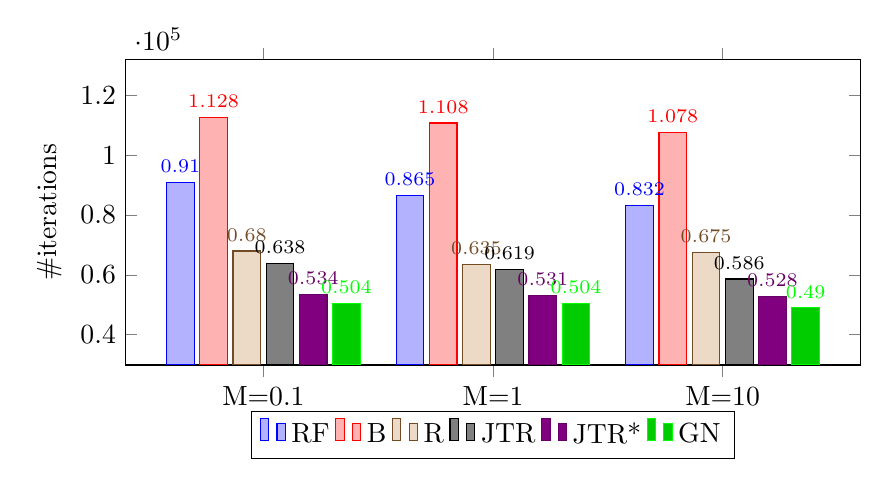
\begin{tikzpicture}
\begin{axis}[
    width=0.9\textwidth,
    height=0.45\textwidth,
    ybar,
    enlargelimits=0.3,
    legend style={at={(0.5,-0.15)},
      anchor=north,legend columns=-1},
    ylabel={\#iterations},
    symbolic x coords={M=0.1,M=1,M=10},
    xtick=data,
    nodes near coords,
    every node near coord/.append style={
    	font=\scriptsize,
	/pgf/number format/precision=3},
    point meta=y *10^-5
    ]
\addplot coordinates {(M=10,83158) (M=1,86480) (M=0.1,91040)};
\addplot coordinates {(M=10,107758) (M=1,110793) (M=0.1,112777)};
\addplot coordinates {(M=10,67537) (M=1,63510) (M=0.1,67961)};
\addplot coordinates {(M=10,58621) (M=1,61930) (M=0.1,63792)};
\addplot coordinates {(M=10,52802) (M=1,53068) (M=0.1,53450)};
\addplot coordinates {(M=10,48972) (M=1,50383) (M=0.1,50389)};
\legend{RF,B,R,JTR,JTR*,GN}
\end{axis}
\end{tikzpicture}
\caption{Number of iterations spent for six different root finders when solving Case A, see Section \ref{section:caseA}, with viscosity ratio $M = \frac{\mu_w}{\mu_o}$. Root finders: RF (Regula Falsi), B (Brent), R (Ridders), JTR (Jenny Trust Region), JTR* (Approximate Jenny Trust Region), and GN (Globalized Newton).}
\label{fig:caseA_iterations}
\end{figure}

The total CPU running times are shown as a function of the time step $\Delta t$ for three different viscosity ratios $M$ in Figure \ref{fig:q5_homperm_10}. Again we include different $M$ values. With $M = 0.1$ all methods have similar performance up to around $\Delta t = \unit[20]{d}$. At this point the regula falsi method, and a little later also the approximate trust region scheme, starts to spend more CPU time than the other methods. This trend is consistent over all subsequent time step sizes. We note that the other methods has equal performance for all time steps.
Next, $M = 1$ gives a similar picture, but here the globalized Newton scheme breaks away at $\Delta t = \unit[10]{days}$ where it starts to slow down compared to the other methods. All the other methods uses equal CPU time over the whole range of time steps.
Finally, $M = 10$ gives the results in Figure \ref{fig:q5_homperm_viscrat_10}. In this case the regula falsi is faster than all the other methods for $\Delta t \gtrapprox \unit[20]{d}$. Further we observe that the Ridders and Brent methods break of last at $\Delta t \approx \unit[20]{d}$, while the trust region scheme breaks of at $\Delta t \approx \unit[5]{d}$, and the approximate trust region scheme and the globalized Newton method does the same at $\Delta t \approx \unit[10]{d}$.

\begin{figure}[!ht]
\centering
\tikzsetnextfilename{q5_hom_m-0_1}
\begin{subfigure}[b]{0.8\textwidth}
\begin{tikzpicture}
    \begin{semilogyaxis}[
            width=0.97\textwidth,
            height=0.26\textheight,
            xlabel={dt~[days]},
            ylabel={CPU time~[s]},
            grid=major,
            ]
        \addplot table[col sep=comma, trim cells=true,x=dt, y=cputime] {datafiles/q5-cputvsdt-s-r-T-300-m-1-10-dim-120-120-20-20-perm-h-10-i-180.data};
        \addplot table[col sep=comma, trim cells=true,x=dt, y=cputime] {datafiles/q5-cputvsdt-s-t-T-300-m-1-10-dim-120-120-20-20-perm-h-10-i-180.data};
        \addplot table[col sep=comma, trim cells=true,x=dt, y=cputime] {datafiles/q5-cputvsdt-s-a-T-300-m-1-10-dim-120-120-20-20-perm-h-10-i-180.data};
        \addplot table[col sep=comma, trim cells=true,x=dt, y=cputime] {datafiles/q5-cputvsdt-s-b-T-300-m-1-10-dim-120-120-20-20-perm-h-10-i-180.data};
        \addplot table[col sep=comma, trim cells=true,x=dt, y=cputime] {datafiles/q5-cputvsdt-s-i-T-300-m-1-10-dim-120-120-20-20-perm-h-10-i-180.data};
                \addplot table[col sep=comma, trim cells=true,x=dt, y=cputime] {datafiles/q5-cputvsdt-s-g-T-300-m-1-10-dim-120-120-20-20-perm-h-10-i-180.data};
        \legend{RF,TR,TR*,B,R,GN}
    \end{semilogyaxis}
\end{tikzpicture}%
\caption{$M =0.1$} \label{fig:q5_homperm_viscrat_0_1}
\end{subfigure}%
\vspace{0.3cm}
\centering
\tikzsetnextfilename{q5_hom_m-1_0}
\begin{subfigure}[b]{0.8\textwidth}
\begin{tikzpicture}
    \begin{semilogyaxis}[
            width=0.97\textwidth,
            height=0.26\textheight,
            xlabel={dt~[days]},
            ylabel={CPU time~[s]},
            grid=major,
            ]
         \addplot table[col sep=comma, trim cells=true,x=dt, y=cputime] {datafiles/q5-cputvsdt-s-r-T-300-m-1-1-dim-120-120-20-20-perm-h-10-i-180.data};
        \addplot table[col sep=comma, trim cells=true,x=dt, y=cputime] {datafiles/q5-cputvsdt-s-t-T-300-m-1-1-dim-120-120-20-20-perm-h-10-i-180.data};
        \addplot table[col sep=comma, trim cells=true,x=dt, y=cputime] {datafiles/q5-cputvsdt-s-a-T-300-m-1-1-dim-120-120-20-20-perm-h-10-i-180.data};
        \addplot table[col sep=comma, trim cells=true,x=dt, y=cputime] {datafiles/q5-cputvsdt-s-b-T-300-m-1-1-dim-120-120-20-20-perm-h-10-i-180.data};
        \addplot table[col sep=comma, trim cells=true,x=dt, y=cputime] {datafiles/q5-cputvsdt-s-i-T-300-m-1-1-dim-120-120-20-20-perm-h-10-i-180.data};
                \addplot table[col sep=comma, trim cells=true,x=dt, y=cputime] {datafiles/q5-cputvsdt-s-g-T-300-m-1-1-dim-120-120-20-20-perm-h-10-i-180.data};
        \legend{RF,TR,TR*,B,R,GN}
    \end{semilogyaxis}
\end{tikzpicture}%
\caption{$M =1$} \label{fig:q5_homperm_viscrat_1}
\end{subfigure}%
\vspace{0.3cm}
\centering
\tikzsetnextfilename{q5_hom_m-10_0}
\begin{subfigure}[b]{0.8\textwidth}
\begin{tikzpicture}
    \begin{semilogyaxis}[
            width=0.97\textwidth,
            height=0.26\textheight,
            xlabel={dt~[days]},
            ylabel={CPU time~[s]},
            grid=major,
            ]
         \addplot table[col sep=comma, trim cells=true,x=dt, y=cputime] {datafiles/q5-cputvsdt-s-r-T-300-m-10-1-dim-120-120-20-20-perm-h-10-i-180.data};
        \addplot table[col sep=comma, trim cells=true,x=dt, y=cputime] {datafiles/q5-cputvsdt-s-t-T-300-m-10-1-dim-120-120-20-20-perm-h-10-i-180.data};
        \addplot table[col sep=comma, trim cells=true,x=dt, y=cputime] {datafiles/q5-cputvsdt-s-a-T-300-m-10-1-dim-120-120-20-20-perm-h-10-i-180.data};
        \addplot table[col sep=comma, trim cells=true,x=dt, y=cputime] {datafiles/q5-cputvsdt-s-b-T-300-m-10-1-dim-120-120-20-20-perm-h-10-i-180.data};
        \addplot table[col sep=comma, trim cells=true,x=dt, y=cputime] {datafiles/q5-cputvsdt-s-i-T-300-m-10-1-dim-120-120-20-20-perm-h-10-i-180.data};
                \addplot table[col sep=comma, trim cells=true,x=dt, y=cputime] {datafiles/q5-cputvsdt-s-g-T-300-m-10-1-dim-120-120-20-20-perm-h-10-i-180.data};
        \legend{RF,TR,TR*,B,R,GN}
    \end{semilogyaxis}
\end{tikzpicture}%
\caption{$M =10$} \label{fig:q5_homperm_viscrat_10}
\end{subfigure}%
\caption{CPU time used to solve the Q5 problem, Section \ref{section:caseA}, for varying root finders, time steps and viscosity ratios.}
\label{fig:q5_homperm_10}
\end{figure}

\subsubsection{Discussion}
A comparison of the iteration count and total CPU time results for test case A, shown in Figure \ref{fig:caseA_iterations} and \ref{fig:q5_homperm_10}, respectively, highlights the differences in computational complexity for the different root finders. That is, even with the quite significant variation in total amount of iterations the CPU time is comparable for all root finders over the range of tested parameters. For instance, the trust region methods, which are essentially Newton methods, converge fast in terms of number of iterations due to the quadratic convergence of the Newton-Raphson scheme. But, since each iteration requires two function evaluations, one for the function itself and one for the derivative, the gains in iterations are balanced by a high overhead in each iteration. Similarly, the Brent method has ``only'' superlinear convergence and thus uses a very high number of iterations, but since it requires just one function evaluation per iteration the total CPU time spent is again normalized. Similar considerations can be used to explain the iteration count versus CPU time results for the other root finders.

\begin{itemize}
\item NB: The following observations are from simulation with $\Delta t = \unit[50]{d}$!
\item The mean size and standard deviation of $| S_r - S_0 |$ correlates with $M$; smaller $M$ gives smaller initial guess errors, larger $M$ gives larger error.
\item $M = 0.1$: Regula falsi experiences one sided convergence quite often. Also the root is often on a very flat part of the residual, giving slow convergence. The regula falsi might benefit from two better initial guesses?
\item $M = 10$: Regula falsi hits more curved regions, giving better convergence. 
\end{itemize}

\clearpage
%%%%%%%%%%%%%%  TARBERT 2D  %%%%%%%%%%%%%%%%%%%
\subsection{Case B: Tarbert 2D}
\label{section:caseB}
The Q5 problem is used again but with a more realistic inhomogeneous permeability distribution taken from the second SPE10 data set \citep{spe10_2000}. The residuals resulting from such permeability distributions typically have different characteristics than the ``homogeneous residuals'' some of which might favor different root finders. The second SPE10 data set consists of scalar permeabilities in the $x$-, $y$- and $z$-directions on a three dimensional grid with $60\times 220\times 85$ cells, with the top 35 layers being part of the Tarbert formation and the bottom 50 the Upper Ness formation.The fine scale permeability grid cells are $\unit[20]{ft}\times \unit[10]{ft}\times \unit[2]{ft}$ in size. Figure \ref{fig:spe10_perm} shows the logarithm of the x-direction permeabilities for the entire domain, from which the $\unit[120]{m}\times \unit[120]{m}$ region starting at $(x,y) = (0,0)$ in the first layer of the Tarbert formation is chosen for the numerical tests.

\begin{figure}[ht]
\centering
\begin{subfigure}{0.49\textwidth}
\includegraphics[width=\textwidth]{figures/saturation_tarbert_layer-0.png}
\caption{Saturation at $T = \unit[30]{d}$}
\label{fig:saturation_tarbert_layer-0}
\end{subfigure}
~
\begin{subfigure}{0.49\textwidth}
\includegraphics[width=\textwidth]{figures/perm_tarbert_layer-0.png}
\caption{Permeability}
\label{fig:perm_tarbert_layer-0}
\end{subfigure}
\caption{}
\label{fig:tarbert_layer-0}
\end{figure}
\tikzsetnextfilename{caseB_iterations}
\begin{figure}[ht]
\centering
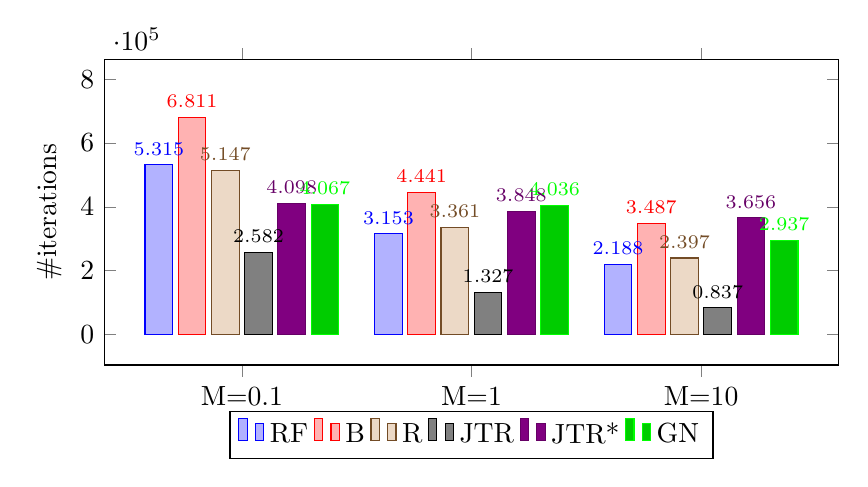
\begin{tikzpicture}
\begin{axis}[
    width=0.9\textwidth,
    height=0.45\textwidth,
    ybar,
    enlargelimits=0.3,
    legend style={at={(0.5,-0.15)},
      anchor=north,legend columns=-1},
    ylabel={\#iterations},
    symbolic x coords={M=0.1,M=1,M=10},
    xtick=data,
    nodes near coords,
    every node near coord/.append style={
    	font=\scriptsize,
	/pgf/number format/precision=3},
    point meta=y *10^-5
    ]
\addplot coordinates {(M=10,218818) (M=1,315318) (M=0.1,531531)};
\addplot coordinates {(M=10,348724) (M=1,444101) (M=0.1,681144)};
\addplot coordinates {(M=10,239669) (M=1,336078) (M=0.1,514705)};
\addplot coordinates {(M=10,83663) (M=1,132662) (M=0.1,258193)};
\addplot coordinates {(M=10,365579) (M=1,384826) (M=0.1,409835)};
\addplot coordinates {(M=10,293725) (M=1,403569) (M=0.1,406730)};
\legend{RF,B,R,JTR,JTR*,GN}
\end{axis}
\end{tikzpicture}
\caption{Number of iterations spent for six different root finders when solving Case B, see Section \ref{section:caseA}, with viscosity ratio $M = \frac{\mu_w}{\mu_o}$. Root finders: RF (Regula Falsi), B (Brent), R (Ridders), JTR (Jenny Trust Region), JTR* (Approximate Jenny Trust Region), and GN (Globalized Newton).}
\label{fig:caseB_iterations}
\end{figure}
\begin{figure}[!ht]
\centering
\tikzsetnextfilename{tarbert_2D_m-0_1}
\begin{subfigure}[b]{0.8\textwidth}
\begin{tikzpicture}
    \begin{semilogyaxis}[
            width=0.97\textwidth,
            height=0.26\textheight,
            xlabel={dt~[days]},
            ylabel={CPU time~[s]},
            grid=major,
            ]
        \addplot table[col sep=comma, trim cells=true,x=dt, y expr= \thisrow{cputime}] {datafiles/spe10-cputvsdt-s-r-T-30-m-1-10-dim-60-60-10-60-220-1-perm-i-0-0-0-i-50.data};
        \addplot table[col sep=comma, trim cells=true,x=dt, y expr=\thisrow{cputime}] {datafiles/spe10-cputvsdt-s-t-T-30-m-1-10-dim-60-60-10-60-220-1-perm-i-0-0-0-i-50.data};
        \addplot table[col sep=comma, trim cells=true,x=dt, y expr=\thisrow{cputime}] {datafiles/spe10-cputvsdt-s-a-T-30-m-1-10-dim-60-60-10-60-220-1-perm-i-0-0-0-i-50.data};
        \addplot table[col sep=comma, trim cells=true,x=dt, y expr=\thisrow{cputime}] {datafiles/spe10-cputvsdt-s-b-T-30-m-1-10-dim-60-60-10-60-220-1-perm-i-0-0-0-i-50.data};
        \addplot table[col sep=comma, trim cells=true,x=dt, y expr=\thisrow{cputime}] {datafiles/spe10-cputvsdt-s-i-T-30-m-1-10-dim-60-60-10-60-220-1-perm-i-0-0-0-i-50.data};
        %\addplot table[col sep=comma, trim cells=true,x=dt, y expr=\thisrow{cputime}] {datafiles/spe10-cputvsdt-s-g-T-30-m-1-10-dim-60-60-10-60-220-1-perm-i-0-0-0-i-50.data};
        \legend{RF,TR,TR*,B,R}
    \end{semilogyaxis}
\end{tikzpicture}%
\label{fig:tarbert_2d_viscrat_0_1}
\caption{Viscosity ratio 0.1}
\end{subfigure}%
\vspace{0.3cm}
\tikzsetnextfilename{tarbert_2D_m-1_0}
\begin{subfigure}[b]{0.8\textwidth}
\begin{tikzpicture}
    \begin{semilogyaxis}[
            width=0.97\textwidth,
            height=0.26\textheight,
            xlabel={dt~[days]},
            ylabel={CPU time~[s]},
            grid=major,
            ]
         \addplot table[col sep=comma, trim cells=true,x=dt, y expr= \thisrow{cputime}] {datafiles/spe10-cputvsdt-s-r-T-30-m-1-1-dim-60-60-10-60-220-1-perm-i-0-0-0-i-50.data};
        \addplot table[col sep=comma, trim cells=true,x=dt, y expr= \thisrow{cputime}] {datafiles/spe10-cputvsdt-s-t-T-30-m-1-1-dim-60-60-10-60-220-1-perm-i-0-0-0-i-50.data};
        \addplot table[col sep=comma, trim cells=true,x=dt, y expr= \thisrow{cputime}] {datafiles/spe10-cputvsdt-s-a-T-30-m-1-1-dim-60-60-10-60-220-1-perm-i-0-0-0-i-50.data};
        \addplot table[col sep=comma, trim cells=true,x=dt, y expr= \thisrow{cputime}] {datafiles/spe10-cputvsdt-s-b-T-30-m-1-1-dim-60-60-10-60-220-1-perm-i-0-0-0-i-50.data};
        \addplot table[col sep=comma, trim cells=true,x=dt, y expr= \thisrow{cputime}] {datafiles/spe10-cputvsdt-s-i-T-30-m-1-1-dim-60-60-10-60-220-1-perm-i-0-0-0-i-50.data};
         %\addplot table[col sep=comma, trim cells=true,x=dt, y expr= \thisrow{cputime}] {datafiles/spe10-cputvsdt-s-g-T-30-m-1-1-dim-60-60-10-60-220-1-perm-i-0-0-0-i-50.data};
        \legend{RF,TR,TR*,B,R}
    \end{semilogyaxis}
\end{tikzpicture}%
\label{fig:tarbert_2d_viscrat_1}
\caption{Viscosity ratio 1}
\end{subfigure}%
\vspace{0.3cm}
\tikzsetnextfilename{tarbert_2D_m-10_0}
\begin{subfigure}[b]{0.8\textwidth}
\begin{tikzpicture}
    \begin{semilogyaxis}[
            width=0.97\textwidth,
            height=0.26\textheight,%
            xlabel={dt~[days]},%
            ylabel={CPU time~[s]},
            grid=major,
            ]
         \addplot table[col sep=comma, trim cells=true,x=dt, y expr= \thisrow{cputime}] {datafiles/spe10-cputvsdt-s-r-T-30-m-10-1-dim-60-60-10-60-220-1-perm-i-0-0-0-i-50.data};
        \addplot table[col sep=comma, trim cells=true,x=dt, y expr= \thisrow{cputime}] {datafiles/spe10-cputvsdt-s-t-T-30-m-10-1-dim-60-60-10-60-220-1-perm-i-0-0-0-i-50.data};
        \addplot table[col sep=comma, trim cells=true,x=dt, y expr= \thisrow{cputime}] {datafiles/spe10-cputvsdt-s-a-T-30-m-10-1-dim-60-60-10-60-220-1-perm-i-0-0-0-i-50.data};
        \addplot table[col sep=comma, trim cells=true,x=dt, y expr= \thisrow{cputime}] {datafiles/spe10-cputvsdt-s-b-T-30-m-10-1-dim-60-60-10-60-220-1-perm-i-0-0-0-i-50.data};
        \addplot table[col sep=comma, trim cells=true,x=dt, y expr= \thisrow{cputime}] {datafiles/spe10-cputvsdt-s-i-T-30-m-10-1-dim-60-60-10-60-220-1-perm-i-0-0-0-i-50.data};
        %\addplot table[col sep=comma, trim cells=true,x=dt, y expr= \thisrow{cputime}] {datafiles/spe10-cputvsdt-s-g-T-30-m-10-1-dim-60-60-10-60-220-1-perm-i-0-0-0-i-50.data};
        \legend{RF,TR,TR*,B,R}
    \end{semilogyaxis}
\end{tikzpicture}%
\label{fig:tarbert_2d_viscrat_10}
\caption{Viscosity ratio 10}
\end{subfigure}%
\label{fig:tarbert_2d}
\caption{CPU time per cell versus time step size $\Delta t$. Inhomogeneous permeabilities from the top layer of the Tarbert formation, as shown in Figure \ref{fig:tarbert_layer-0}.}
\end{figure}

\todoinline{Comment the results from Tarbert 2D}

\clearpage
%%%%%%%%%%%%%%%%  UPPER NESS 2D %%%%%%%%%%%%%%%%%%%
\subsection{Case C: Upper Ness 2D}
\label{section:caseC}
Figure \ref{fig:spe10_perm} indicates that the Upper Ness formation has more severe local permeability variations compared to the Tarbert formation. These large local variations appear as \todo{show the effects of large local perm. gradients on the residual.}. Again we want to investigate how the various root finders perform on this special case, choosing the $\unit[360]{m}\times \unit[180]{m}$ region starting at $(x,y) = (0,0)$ in layer 45 of the SPE10 data set for the permeabilities.

\begin{figure}[ht]
\centering
\begin{subfigure}{0.49\textwidth}
\includegraphics[width=\textwidth]{figures/saturation_upperness_layer-35.png}
\caption{Saturation at $T = \unit[30]{d}$}
\label{fig:saturation_upperness_layer-35}
\end{subfigure}
~
\begin{subfigure}{0.49\textwidth}
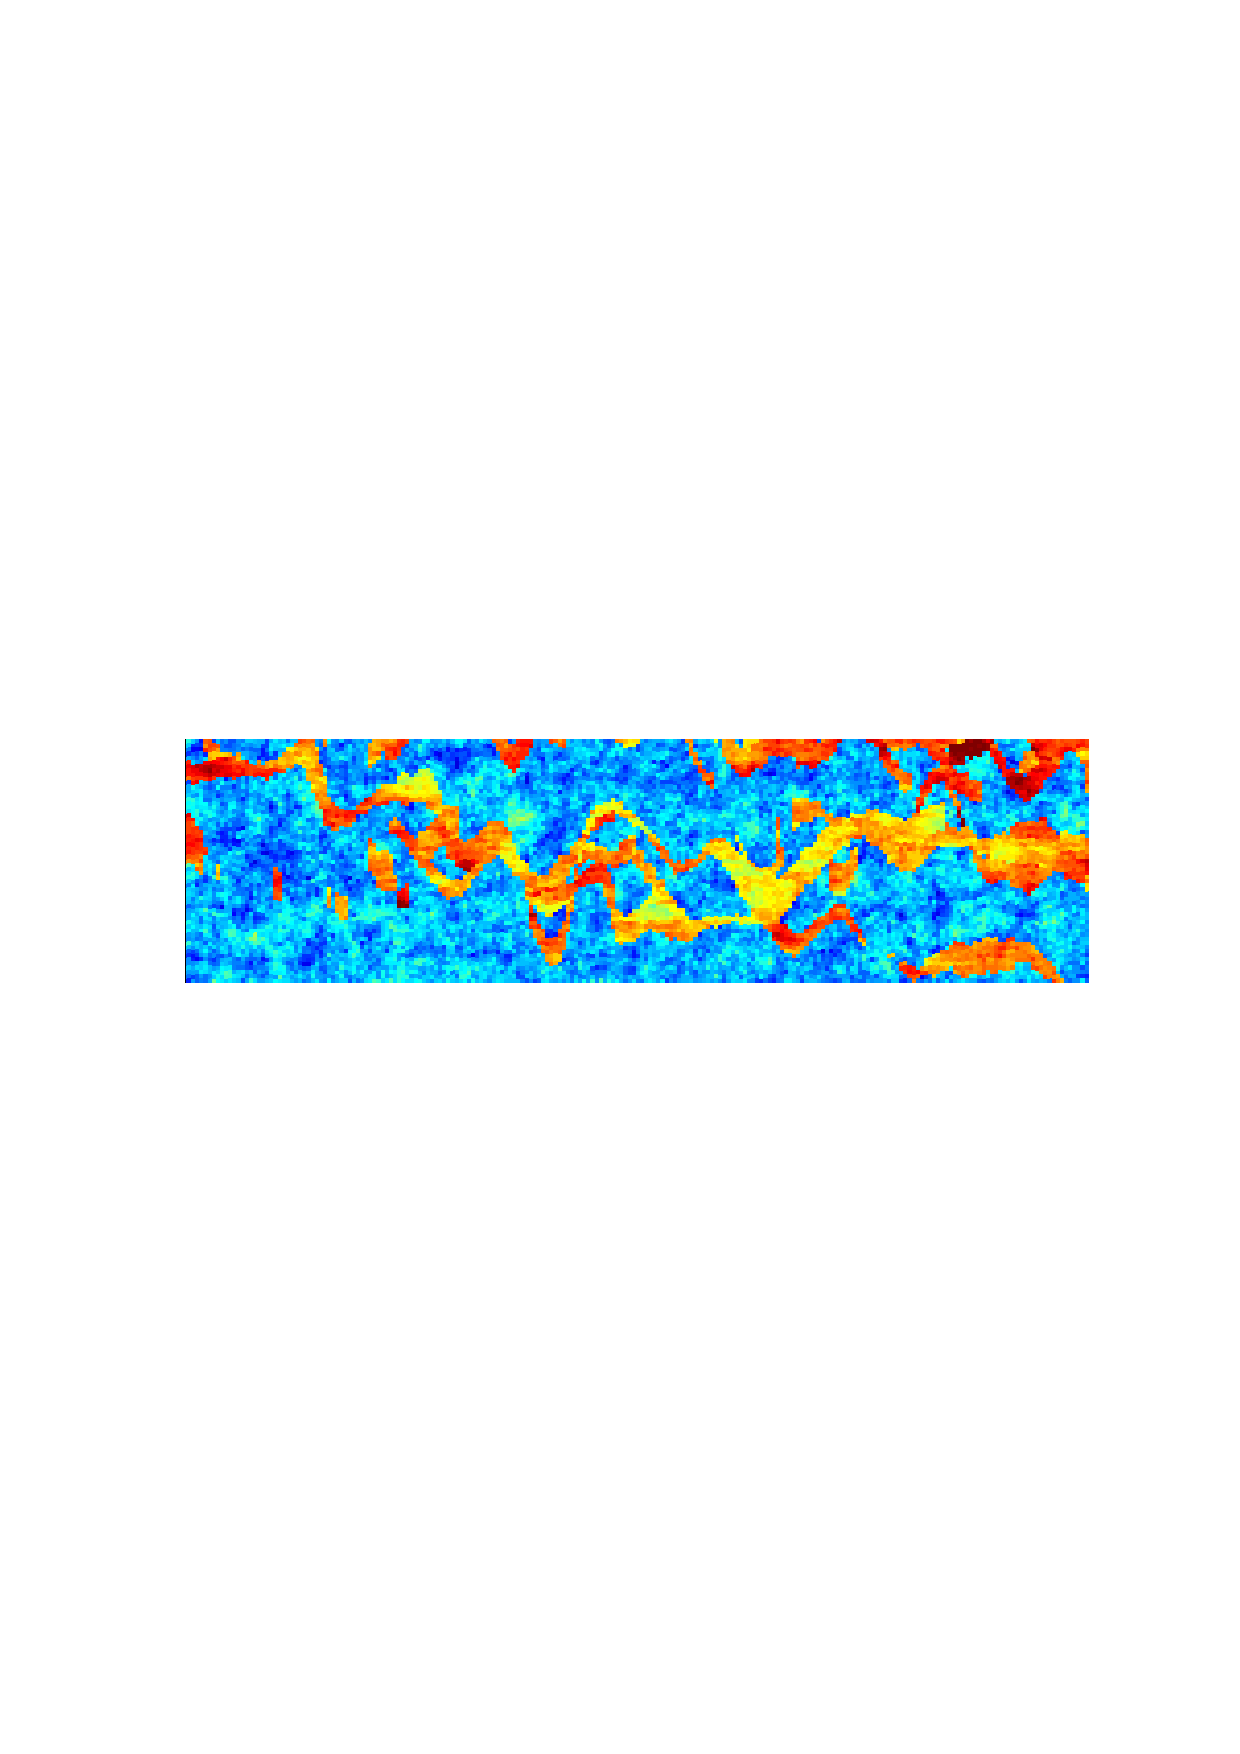
\includegraphics[width=\textwidth]{figures/perm_upperness_layer-35.png}
\caption{Permeability}
\label{fig:perm_upperness_layer-35}
\end{subfigure}
\caption{}
\label{fig:upperness_layer-35}
\end{figure}
\tikzsetnextfilename{caseC_iterations}
\begin{figure}[ht]
\centering
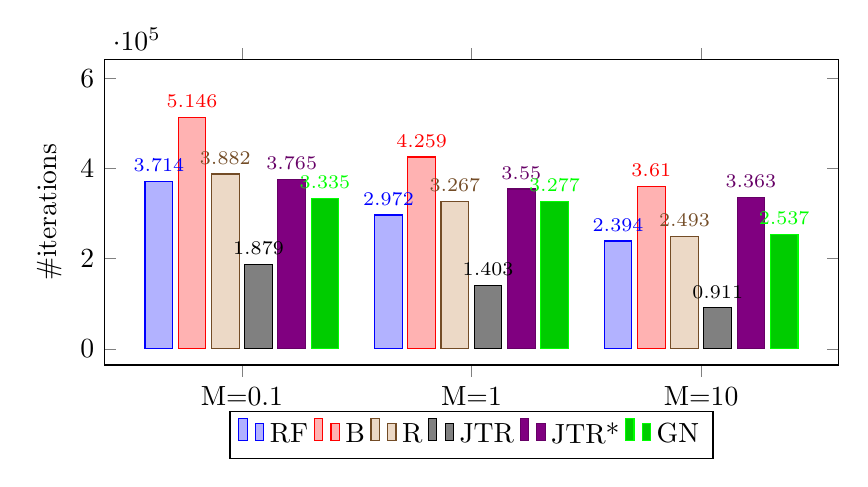
\begin{tikzpicture}
\begin{axis}[
    width=0.9\textwidth,
    height=0.45\textwidth,
    ybar,
    enlargelimits=0.3,
    legend style={at={(0.5,-0.15)},
      anchor=north,legend columns=-1},
    ylabel={\#iterations},
    symbolic x coords={M=0.1,M=1,M=10},
    xtick=data,
    nodes near coords,
    every node near coord/.append style={
    	font=\scriptsize,
	/pgf/number format/precision=3},
    point meta=y *10^-5
    ]
\addplot coordinates {(M=10,239352) (M=1,297199) (M=0.1,371414)};
\addplot coordinates {(M=10,360967) (M=1,425877) (M=0.1,514572)};
\addplot coordinates {(M=10,249254) (M=1,326676) (M=0.1,388250)};
\addplot coordinates {(M=10,91061) (M=1,140320) (M=0.1,187857)};
\addplot coordinates {(M=10,336270) (M=1,355013) (M=0.1,376547)};
\addplot coordinates {(M=10,253670) (M=1,327701) (M=0.1,333513)};
\legend{RF,B,R,JTR,JTR*,GN}
\end{axis}
\end{tikzpicture}
\caption{Number of iterations spent for six different root finders when solving Case C, see Section \ref{section:caseA}, with viscosity ratio $M = \frac{\mu_w}{\mu_o}$. Root finders: RF (Regula Falsi), B (Brent), R (Ridders), JTR (Jenny Trust Region), JTR* (Approximate Jenny Trust Region), and GN (Globalized Newton).}
\label{fig:caseC_iterations}
\end{figure}
\input{spe10-cputvsdt-s-x-T-30-m-x-dim-60-60-10-60-220-1-perm-i-36-0-0-i-50}

\todoinline{Comment the results from Upper Ness 2D}

\clearpage
%%%%%%%%%%%%%%%% TARBERT - 3D %%%%%%%%%%%%%%%%%%%
\subsection{Case D: Tarbert 3D}
\label{section:caseD}

\todoinline{Permeability/saturation plot for Tarbert 3D}
\todoinline{Run Tarbert 3D with gravity - cputime}
\todoinline{Run Tarbert 3D with gravity - iterations}

\clearpage
%%%%%%%%%%%%%%%%  UPPER NESS - 3D %%%%%%%%%%%%%%%%%%%
\subsection{Case E: Upper Ness 3D}
\label{section:caseE}

\todoinline{Permeability/saturation plot for Upper Ness 3D}
\todoinline{Run Upper Ness 3D with gravity - cputime}
\todoinline{Run Upper Ness 3D with gravity - iterations}

\clearpage
%%%%%%%%%%%%%%%% CONVERGENCE TESTS %%%%%%%%%%%%%%%%%%
\section{Convergence Tests}
\label{section:numerical_results_convergence_tests}
The efficiency of the numerical methods in terms of convergence speed can highlight the properties of the numerical procedures. We again \todo{Comment briefly on the properties of the viscosity residual when it is introduced.} observe that the form of the viscosity dominated residual from Equation (\ref{eq:residual_two_phase_transport}) is determined by five parameters; the initial saturation in the cell, $S_V^{n}$, the time step to pore volume ratio $\tau = \frac{\Delta t}{m(V)\phi_V}$, the flux out of the cell $q_o$, the flux into the cell $q_i$, and finally the viscosity ratio $M$ as defined in Equation (\ref{eq:viscosity_ratio}), held constant at $M = 1$. Note that the cell saturation from the previous time step is used as initial guess for the root finders. Figures \ref{fig:conv_res_in_0_05_out_0_05} through \ref{fig:conv_res_in_0_5_out_0_8} shows a number of different convergence and residual plots obtained by varying these parameters. 

Figure \ref{fig:conv_res_in_0_05_out_0_05} is obtained with incoming flux at $\unitfrac[0.05]{m^3}{s}$ and outgoing flux at $\unitfrac[0.05]{m^3}{s}$. Note that $\tau = \unitfrac[6]{s}{m^3}$. Under the circumstances the residuals are fairly linear, and the initial guess $S_0$ is close to the root. The number of iterations for all tested root finders decreases when $S_0$ is increased. We also note that the Newton-like methods converge faster than the other methods. This plot indicates that for small flux values the initial guess strongly influences the residual bringing the root close to $S_0$. with a stronger effect for larger $S_0$. 

Setting the incoming flux to $\unitfrac[0.35]{m^3}{s}$ and the outgoing flux to $\unitfrac[0.35]{m^3}{s}$ we obtain Figure \ref{fig:conv_res_in_0_35_out_0_35}. The residual plots shown a stronger non-linear influence, a fact reflected in the increased iteration count. $S_0$ still influences the residual, but to a lesser extent. Again we observe that large initial guesses generally leads to a lower iteration count. The Newton-like method are, together with Ridders, the best performers.

Moving on the even larger flux values, we set the incoming flux to $\unitfrac[0.5]{m^3}{s}$ and the outgoing flux to $\unitfrac[0.8]{m^3}{s}$. Figure \ref{fig:conv_res_in_0_5_out_0_8} shows the resulting plots. The trend from the previous plots continues, in that the initial guess has less influence on the performance of the root finders, on average. Interesting exceptions are the Newton-like methods. They perform significantly better in terms of iteration count when the initial guess is close, in contrast with the other methods. We also note that the initial has very little influence on the position of the root.

\input{convergence2-s-x-M-1_000000-dtpv-6_000000-in--0_050000-out-0_050000-s0-x}
\begin{figure}[!ht]
\centering
\begin{subfigure}[b]{0.49\textwidth}
\begin{tikzpicture}
    \begin{semilogyaxis}[
            width=0.97\textwidth,
            height=0.3\textheight,
            xlabel={\#steps},
            ylabel={error},
            grid=both,
            legend pos=south west,
            ]
        \addplot table[col sep=comma, trim cells=true,x=iter, y=y] {testcasedatafiles/convergence2-s-r-M-1_000000-dtpv-6_000000-in--0_350000-out-0_350000-s0-0_100000.data};
        \addplot table[col sep=comma, trim cells=true,x=iter, y=y] {testcasedatafiles/convergence2-s-t-M-1_000000-dtpv-6_000000-in--0_350000-out-0_350000-s0-0_100000.data};
        \addplot table[col sep=comma, trim cells=true,x=iter, y=y] {testcasedatafiles/convergence2-s-a-M-1_000000-dtpv-6_000000-in--0_350000-out-0_350000-s0-0_100000.data};
        \addplot table[col sep=comma, trim cells=true,x=iter, y=y] {testcasedatafiles/convergence2-s-b-M-1_000000-dtpv-6_000000-in--0_350000-out-0_350000-s0-0_100000.data};
        \addplot table[col sep=comma, trim cells=true,x=iter, y=y] {testcasedatafiles/convergence2-s-i-M-1_000000-dtpv-6_000000-in--0_350000-out-0_350000-s0-0_100000.data};
        \addplot table[col sep=comma, trim cells=true,x=iter, y=y] {testcasedatafiles/convergence2-s-g-M-1_000000-dtpv-6_000000-in--0_350000-out-0_350000-s0-0_100000.data};
        \legend{RF,TR,TR*,B,R,GN}
    \end{semilogyaxis}
\end{tikzpicture}%
\caption{$S_0 = 0.1$}
\label{fig:convergence_in_0_35_out_0_35_s0_0_1}
\end{subfigure}%
\begin{subfigure}[b]{0.49\textwidth}
\begin{tikzpicture}
    \begin{axis}[
            width=0.97\textwidth,
            height=0.3\textheight,
            xlabel={S},
            ylabel={$R(S)$},
            grid=both,
            legend pos=north west,
            ]
        \addplot table[mark=none, col sep=comma, trim cells=true,x=s, y=Rs] {testcasedatafiles/residual-convergence2-s-r-M-1_000000-dtpv-6_000000-in--0_350000-out-0_350000-s0-0_100000.data};
        \addplot table[mark=none, col sep=comma, trim cells=true,x=s, y=dRs] {testcasedatafiles/residual-convergence2-s-r-M-1_000000-dtpv-6_000000-in--0_350000-out-0_350000-s0-0_100000.data};
            \legend{$R(S)$,$\partial_S R(S)$}
    \end{axis}
\end{tikzpicture}%
\caption{$S_0 = 0.1$}
\label{fig:residual_in_0_35_out_0_35_s0_0_1}
\end{subfigure}%
\vspace{0.4cm}
\begin{subfigure}[b]{0.49\textwidth}
\begin{tikzpicture}
    \begin{semilogyaxis}[
            width=0.97\textwidth,
            height=0.3\textheight,
            xlabel={\#steps},
            ylabel={error},
            grid=both,
            legend pos=south west,
            ]
        \addplot table[col sep=comma, trim cells=true,x=iter, y=y] {testcasedatafiles/convergence2-s-r-M-1_000000-dtpv-6_000000-in--0_350000-out-0_350000-s0-0_500000.data};
        \addplot table[col sep=comma, trim cells=true,x=iter, y=y] {testcasedatafiles/convergence2-s-t-M-1_000000-dtpv-6_000000-in--0_350000-out-0_350000-s0-0_500000.data};
        \addplot table[col sep=comma, trim cells=true,x=iter, y=y] {testcasedatafiles/convergence2-s-a-M-1_000000-dtpv-6_000000-in--0_350000-out-0_350000-s0-0_500000.data};
        \addplot table[col sep=comma, trim cells=true,x=iter, y=y] {testcasedatafiles/convergence2-s-b-M-1_000000-dtpv-6_000000-in--0_350000-out-0_350000-s0-0_500000.data};
        \addplot table[col sep=comma, trim cells=true,x=iter, y=y] {testcasedatafiles/convergence2-s-i-M-1_000000-dtpv-6_000000-in--0_350000-out-0_350000-s0-0_500000.data};
        \addplot table[col sep=comma, trim cells=true,x=iter, y=y] {testcasedatafiles/convergence2-s-g-M-1_000000-dtpv-6_000000-in--0_350000-out-0_350000-s0-0_500000.data};
        \legend{RF,TR,TR*,B,R,GN}
    \end{semilogyaxis}
\end{tikzpicture}%
\caption{$S_0 = 0.5$}
\label{fig:convergence_in_0_35_out_0_35_s0_0_5}
\end{subfigure}%
\begin{subfigure}[b]{0.49\textwidth}
\begin{tikzpicture}
    \begin{axis}[
            width=0.97\textwidth,
            height=0.3\textheight,
            xlabel={S},
            ylabel={$R(S)$},
            grid=both,
            legend pos=north west,
            ]
        \addplot table[mark=none, col sep=comma, trim cells=true,x=s, y=Rs] {testcasedatafiles/residual-convergence2-s-r-M-1_000000-dtpv-6_000000-in--0_350000-out-0_350000-s0-0_500000.data};
        \addplot table[mark=none, col sep=comma, trim cells=true,x=s, y=dRs] {testcasedatafiles/residual-convergence2-s-r-M-1_000000-dtpv-6_000000-in--0_350000-out-0_350000-s0-0_500000.data};
            \legend{$R(S)$,$\partial_S R(S)$}
    \end{axis}
\end{tikzpicture}%
\caption{$S_0 = 0.5$}
\label{fig:residual_in_0_35_out_0_35_s0_0_5}
\end{subfigure}%
\vspace{0.4cm}
\begin{subfigure}[b]{0.49\textwidth}
\begin{tikzpicture}
    \begin{semilogyaxis}[
            width=0.97\textwidth,
            height=0.3\textheight,
            xlabel={\#steps},
            ylabel={error},
            grid=both,
            legend pos=south west,
            ]
        \addplot table[col sep=comma, trim cells=true,x=iter, y=y] {testcasedatafiles/convergence2-s-r-M-1_000000-dtpv-6_000000-in--0_350000-out-0_350000-s0-0_900000.data};
        \addplot table[col sep=comma, trim cells=true,x=iter, y=y] {testcasedatafiles/convergence2-s-t-M-1_000000-dtpv-6_000000-in--0_350000-out-0_350000-s0-0_900000.data};
        \addplot table[col sep=comma, trim cells=true,x=iter, y=y] {testcasedatafiles/convergence2-s-a-M-1_000000-dtpv-6_000000-in--0_350000-out-0_350000-s0-0_900000.data};
        \addplot table[col sep=comma, trim cells=true,x=iter, y=y] {testcasedatafiles/convergence2-s-b-M-1_000000-dtpv-6_000000-in--0_350000-out-0_350000-s0-0_900000.data};
        \addplot table[col sep=comma, trim cells=true,x=iter, y=y] {testcasedatafiles/convergence2-s-i-M-1_000000-dtpv-6_000000-in--0_350000-out-0_350000-s0-0_900000.data};
        \addplot table[col sep=comma, trim cells=true,x=iter, y=y] {testcasedatafiles/convergence2-s-g-M-1_000000-dtpv-6_000000-in--0_350000-out-0_350000-s0-0_900000.data};
        \legend{RF,TR,TR*,B,R,GN}
    \end{semilogyaxis}
\end{tikzpicture}%
\caption{$S_0 = 0.9$}
\label{fig:convergence_in_0_35_out_0_35_s0_0_9}
\end{subfigure}%
\begin{subfigure}[b]{0.49\textwidth}
\begin{tikzpicture}
    \begin{axis}[
            width=0.97\textwidth,
            height=0.3\textheight,
            xlabel={S},
            ylabel={$R(S)$},
            grid=both,
            legend pos=north west,
            ]
        \addplot table[mark=none, col sep=comma, trim cells=true,x=s, y=Rs] {testcasedatafiles/residual-convergence2-s-r-M-1_000000-dtpv-6_000000-in--0_350000-out-0_350000-s0-0_900000.data};
        \addplot table[mark=none, col sep=comma, trim cells=true,x=s, y=dRs] {testcasedatafiles/residual-convergence2-s-r-M-1_000000-dtpv-6_000000-in--0_350000-out-0_350000-s0-0_900000.data};
            \legend{$R(S)$,$\partial_S R(S)$}
    \end{axis}
\end{tikzpicture}%
\caption{$S_0 = 0.9$}
\label{fig:residual_in_0_35_out_0_35_s0_0_9}
\end{subfigure}%
\caption{M = 1, dtpv = 6, influx = -0.35, outflux = 0.35}
\label{fig:conv_res_in_0_35_out_0_35}
\end{figure}

\input{convergence2-s-x-M-1_000000-dtpv-6_000000-in--0_500000-out-0_800000-s0-x}

\clearpage
%%%%%%%%%%%%%%%% GRAVITY TESTS %%%%%%%%%%%%%%%%%%
\section{Gravity Tests}
\todoinline{Turn off source/sink and run tests with only gravity effects?}
%\begin{figure}[!ht]
\centering
\tikzsetnextfilename{gravres-cell-0}
\begin{tikzpicture}
    \begin{axis}[
            width=0.97\textwidth,
            height=0.26\textheight,
            xlabel={$S_w$},
            ylabel={$R$},
            grid=major,
            ]
        \addplot table[mark=none,col sep=comma, trim cells=true,x=snp, y=Rnp] {datafiles/gravres-cell-0.data};
        \addplot table[mark=none,col sep=comma, trim cells=true,x=snp, y=dRnp] {datafiles/gravres-cell-0.data};
    \end{axis}
\end{tikzpicture}%
\caption{Gravity residual in cell 0.}
\end{figure}

\begin{figure}[!ht]
\centering
\tikzsetnextfilename{gravres-cell-10}
\begin{tikzpicture}
    \begin{axis}[
            width=0.97\textwidth,
            height=0.26\textheight,
            xlabel={$S_w$},
            ylabel={$R$},
            grid=major,
            ]
        \addplot table[mark=none,col sep=comma, trim cells=true,x=snp, y=Rnp] {datafiles/gravres-cell-10.data};
        \addplot table[mark=none,col sep=comma, trim cells=true,x=snp, y=dRnp] {datafiles/gravres-cell-10.data};
    \end{axis}
\end{tikzpicture}%
\caption{Gravity residual in cell 10.}
\end{figure}


\begin{figure}[!ht]
\centering
\tikzsetnextfilename{gravres-cell-20}
\begin{tikzpicture}
    \begin{axis}[
            width=0.97\textwidth,
            height=0.26\textheight,
            xlabel={$S_w$},
            ylabel={$R$},
            grid=major,
            ]
        \addplot table[mark=none,col sep=comma, trim cells=true,x=snp, y=Rnp] {datafiles/gravres-cell-20.data};
        \addplot table[mark=none,col sep=comma, trim cells=true,x=snp, y=dRnp] {datafiles/gravres-cell-20.data};
    \end{axis}
\end{tikzpicture}%
\caption{Gravity residual in cell 20.}
\end{figure}


\begin{figure}[!ht]
\centering
\tikzsetnextfilename{gravres-cell-30}
\begin{tikzpicture}
    \begin{axis}[
            width=0.97\textwidth,
            height=0.26\textheight,
            xlabel={$S_w$},
            ylabel={$R$},
            grid=major,
            ]
        \addplot table[mark=none,col sep=comma, trim cells=true,x=snp, y=Rnp] {datafiles/gravres-cell-30.data};
        \addplot table[mark=none,col sep=comma, trim cells=true,x=snp, y=dRnp] {datafiles/gravres-cell-30.data};
    \end{axis}
\end{tikzpicture}%
\caption{Gravity residual in cell 30.}
\end{figure}


\begin{figure}[!ht]
\centering
\tikzsetnextfilename{gravres-cell-40}
\begin{tikzpicture}
    \begin{axis}[
            width=0.97\textwidth,
            height=0.26\textheight,
            xlabel={$S_w$},
            ylabel={$R$},
            grid=major,
            ]
        \addplot table[mark=none,col sep=comma, trim cells=true,x=snp, y=Rnp] {datafiles/gravres-cell-40.data};
        \addplot table[mark=none,col sep=comma, trim cells=true,x=snp, y=dRnp] {datafiles/gravres-cell-40.data};
    \end{axis}
\end{tikzpicture}%
\caption{Gravity residual in cell 40.}
\end{figure}

\begin{figure}[!ht]
\centering
\tikzsetnextfilename{gravres-cell-50}
\begin{tikzpicture}
    \begin{axis}[
            width=0.97\textwidth,
            height=0.26\textheight,
            xlabel={$S_w$},
            ylabel={$R$},
            grid=major,
            ]
        \addplot table[mark=none,col sep=comma, trim cells=true,x=snp, y=Rnp] {datafiles/gravres-cell-50.data};
        \addplot table[mark=none,col sep=comma, trim cells=true,x=snp, y=dRnp] {datafiles/gravres-cell-50.data};
    \end{axis}
\end{tikzpicture}%
\caption{Gravity residual in cell 50.}
\end{figure}

\begin{figure}[!ht]
\centering
\tikzsetnextfilename{gravres-cell-60}
\begin{tikzpicture}
    \begin{axis}[
            width=0.97\textwidth,
            height=0.26\textheight,
            xlabel={$S_w$},
            ylabel={$R$},
            grid=major,
            ]
        \addplot table[mark=none,col sep=comma, trim cells=true,x=snp, y=Rnp] {datafiles/gravres-cell-60.data};
        \addplot table[mark=none,col sep=comma, trim cells=true,x=snp, y=dRnp] {datafiles/gravres-cell-60.data};
    \end{axis}
\end{tikzpicture}%
\caption{Gravity residual in cell 60.}
\end{figure}

\begin{figure}[!ht]
\centering
\tikzsetnextfilename{gravres-cell-60}
\begin{tikzpicture}
    \begin{axis}[
            width=0.97\textwidth,
            height=0.26\textheight,
            xlabel={$S_w$},
            ylabel={$R$},
            grid=major,
            ]
        \addplot table[mark=none,col sep=comma, trim cells=true,x=snp, y=Rnp] {datafiles/gravres-cell-70.data};
        \addplot table[mark=none,col sep=comma, trim cells=true,x=snp, y=dRnp] {datafiles/gravres-cell-70.data};
    \end{axis}
\end{tikzpicture}%
\caption{Gravity residual in cell 70.}
\end{figure}

\begin{figure}[!ht]
\centering
\tikzsetnextfilename{gravres-cell-80}
\begin{tikzpicture}
    \begin{axis}[
            width=0.97\textwidth,
            height=0.26\textheight,
            xlabel={$S_w$},
            ylabel={$R$},
            grid=major,
            ]
        \addplot table[mark=none,col sep=comma, trim cells=true,x=snp, y=Rnp] {datafiles/gravres-cell-80.data};
        \addplot table[mark=none,col sep=comma, trim cells=true,x=snp, y=dRnp] {datafiles/gravres-cell-80.data};
    \end{axis}
\end{tikzpicture}%
\caption{Gravity residual in cell 80.}
\end{figure}

\begin{figure}[!ht]
\centering
\tikzsetnextfilename{gravres-cell-90}
\begin{tikzpicture}
    \begin{axis}[
            width=0.97\textwidth,
            height=0.26\textheight,
            xlabel={$S_w$},
            ylabel={$R$},
            grid=major,
            ]
        \addplot table[mark=none,col sep=comma, trim cells=true,x=snp, y=Rnp] {datafiles/gravres-cell-90.data};
        \addplot table[mark=none,col sep=comma, trim cells=true,x=snp, y=dRnp] {datafiles/gravres-cell-90.data};
    \end{axis}
\end{tikzpicture}%
\caption{Gravity residual in cell 90.}
\end{figure}

\begin{figure}[!ht]
\centering
\tikzsetnextfilename{gravres-cell-99}
\begin{tikzpicture}
    \begin{axis}[
            width=0.97\textwidth,
            height=0.26\textheight,
            xlabel={$S_w$},
            ylabel={$R$},
            grid=major,
            ]
        \addplot table[mark=none,col sep=comma, trim cells=true,x=snp, y=Rnp] {datafiles/gravres-cell-99.data};
        \addplot table[mark=none,col sep=comma, trim cells=true,x=snp, y=dRnp] {datafiles/gravres-cell-99.data};
    \end{axis}
\end{tikzpicture}%
\caption{Gravity residual in cell 99.}
\end{figure}
